% Define document type
\documentclass{beamer}

% Include packages
\usepackage[german, english]{babel} % Languages
\usepackage{tikz} % Tikz figures
\usepackage{siunitx} % SI-units package
\usepackage{bm} % Bold mathematics
\usepackage{listings} % Make listings, e.g. for code
\usepackage{enumitem} % Enumerate and itemize commands
\usepackage{multicol} % Make multiple columns for content
\usepackage[left=15mm, right=15mm, bottom=15mm, top=15mm, includeheadfoot]{geometry} % Modify geometry of page format
\usepackage{placeins} % For float barrier command
\usepackage{amsmath} % Math environments
\usepackage{fancyhdr} % Include the fancyhdr package
\usepackage{amsthm} % Theorem environments
\usepackage{siunitx} % Use SI
\usepackage{array} % Use array package for tables
\usepackage{tabularx} % Package to make nice tables
\usepackage{amssymb} % Math symbols
\usepackage{lipsum} % Provide dummy text
\usepackage{abstract} % Abstract package
\usepackage{nicefrac} % Nice fractions in in-line texts
\usepackage[hidelinks]{hyperref} % Make document with hyperlinks
\usepackage{cleveref} % Make references
\usepackage{subcaption} % Make subfigures
\usepackage{graphicx} % Make figures
\usepackage{mhchem} % Chemical notation
\usepackage{mathtools} % Various math tools
\usepackage{framed} % Frame equations

% Include commands
% Figure caption setup
\captionsetup{font=footnotesize,labelfont=bf}

% Python code listings
\definecolor{codegreen}{rgb}{0,0.6,0}
\definecolor{codegray}{rgb}{0.5,0.5,0.5}
\definecolor{codepurple}{rgb}{0.58,0,0.82}
\definecolor{backcolour}{rgb}{0.95,0.95,0.92}

\lstdefinestyle{mystyle}{
	backgroundcolor=\color{backcolour},   
	commentstyle=\color{codegreen},
	keywordstyle=\color{magenta},
	numberstyle=\tiny\color{codegray},
	stringstyle=\color{codepurple},
	basicstyle=\ttfamily\footnotesize,
	breakatwhitespace=false,         
	breaklines=true,                 
	captionpos=b,                    
	keepspaces=true,                 
	numbers=left,                    
	numbersep=5pt,                  
	showspaces=false,                
	showstringspaces=false,
	showtabs=false,                  
	tabsize=2
}

% Enumerate style
\renewcommand{\theenumi}{(\arabic{enumi})}
\renewcommand\labelenumi{\theenumi} % Change enumerate style from 1. to (1) etc.
\renewcommand{\theenumiii}{(\arabic{enumiii})}
\renewcommand\labelenumiii{\theenumiii} % Change enumerate style from 1. to (1) etc.
\setlist{itemsep = 0.2pt}

% Matrix and vector notation
\newcommand\matr[1]{\ensuremath{\boldsymbol{\mathbf{#1}}}}
\newcommand\vect[1]{\ensuremath{\bm{#1}}}
\newcommand\dint{\ensuremath{\int\displaylimits}}

% Units definitions
\DeclareSIUnit \parsec {pc}
\DeclareSIUnit \magnitudes {mag}

% Theorem environment
\newtheorem{tm}{Theorem}
\numberwithin{tm}{subsection}

% New tag form
\newtagform{normalsize}[\normalsize]{\normalsize(}{\normalsize)}

% Configure head- and footlines
\pagestyle{fancy} % Set head- and footlines
\fancyhead[C]{Adult face predicting machine} % Left headline
\fancyhead[L]{\nouppercase{\leftmark}} % Right headline
\fancyhead[R]{D. Zahnd, R. Zahnd}

% Include logos for the title page
\titlegraphic{
  \vspace{-8.4cm}
  
\includegraphics[height=2.0cm]{figures/ublogo.pdf}\hfill
  
\includegraphics[height=1.3cm]{figures/metaslogo.pdf}
  \vspace{2.5cm}
}

% Define title page
\title{The METAS joule-watt balance \\  \vspace{0.4cm} \small A combined approach}
\author{\scriptsize PhD project presentation \\ \vspace{0.5cm} \normalsize Daniel Zahnd}
\date{July 09, 2024}


% Begin document
\begin{document}

\begin{frame}[noframenumbering, plain]
\maketitle
\end{frame}
\setcounter{framenumber}{0}

\setlength{\parskip}{2pt}
\begin{frame}{Content}
\tableofcontents
\end{frame}
\setlength{\parskip}{8pt}

\section{Introduction}
\begin{frame}[allowframebreaks]{Introduction}
\framesubtitle{Background}
\begin{itemize}
    \item The kilogram prototype in Paris is not stable with respect to time.
    \item The watt balance invented by \cite{Kibble1976} provides a constant representation.
    \item The watt balance is nowadays named after its inventor as Kibble balance.
    \item The Kibble balance method is based on a comparison of electrical to mechanical power.
    \end{itemize}
\end{frame}

\begin{frame}[allowframebreaks]{Introduction}
\framesubtitle{Working principle of the watt balance}
  \begin{columns}
    \begin{column}{0.49\textwidth}
    \begin{itemize}
        \item From electrodynamics, the electromagnetic force \begin{equation}\label{eq:electromagnetic_force}
            \vect{F}_{el} = I_s\oint\vect{B}\times \mathrm{d}\vect{l}
        \end{equation} can be derived.
        \item The current $I_s$ is varied such that $\vect{F}_{el} = \vect{F}_g$.
        \item Current $I_s$ and voltage $U_s$ are measured.
    \end{itemize}
    \end{column}
    
    \begin{column}{0.5\textwidth}
      \begin{figure}[h!] 
        		\centering
		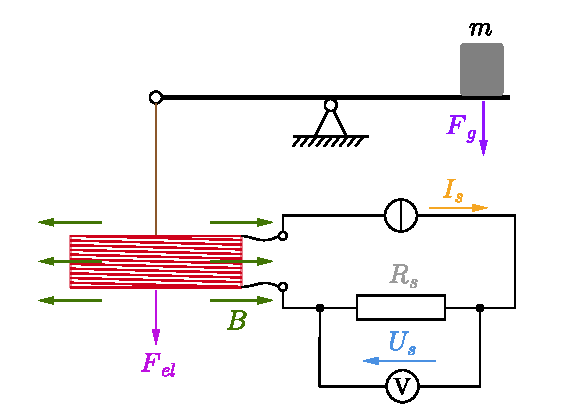
\includegraphics[width=\textwidth]{figures/balancestatic.pdf}
		\caption{Static mode of the Kibble balance.}
		\label{fig:balancestatic}
      \end{figure}
    \end{column}
  \end{columns}
\end{frame}

\begin{frame}[allowframebreaks]{Introduction}
\framesubtitle{Working principle of the watt balance}
  \begin{columns}
    \begin{column}{0.49\textwidth}
    \begin{itemize}
        \item From electrodynamics, the electromagnetic induction \begin{equation}
            \label{eq:electromagnetic_induction}
            U_d = \oint(\vect{B}\times \mathrm{d}\vect{l})\cdot \vect{v}
        \end{equation} can be derived.
    \item The coil is moved at velocity $\vect{v}$.
    \item Induced voltage $U_d$ is measured.
    \end{itemize}
    \end{column}
    
    \begin{column}{0.5\textwidth}
      \begin{figure}[h!] 
		\centering
		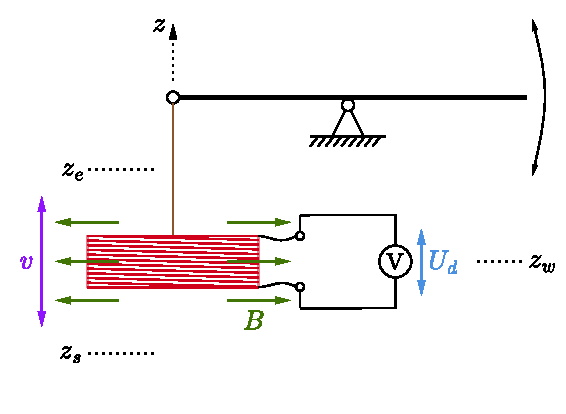
\includegraphics[width=\textwidth]{figures/balancedynamic.pdf}
		\caption{Dynamic mode of the Kibble balance.}
		\label{fig:balancedynamic}
      \end{figure}
    \end{column}
  \end{columns}
\end{frame}

\begin{frame}[allowframebreaks]{Introduction}
\framesubtitle{Working principle of the watt balance}
\begin{itemize}
    \item Bringing \cref{eq:electromagnetic_force} and \cref{eq:electromagnetic_induction} together yields
    \begin{equation}\label{eq:preliminary_equation}
    \left.
    \begin{aligned}
    \vect{F}_{el} = I_s\oint\vect{B}&\times \mathrm{d}\vect{l} = m\vect{g}  \\
    U_d = \oint (\vect{B}&\times \mathrm{d}\vect{l})\cdot \vect{v}
    \end{aligned}  \quad \right\} \quad  m\vect{g}\cdot\vect{v} = U_dI_s.
\end{equation}
\item The voltage $U_d$ and the resistance $I_s$ are related to the Planck constant $h$ by means of the quantum Hall and Josephson effects, namely \begin{equation}\label{eq:planck_relations}
    U_d = C_dn_{J,d}f_{J,d}\frac{h}{2e}, \qquad I_s = C_sn_{J,s}f_{J,s}\frac{n_He}{2}.
\end{equation}
\end{itemize}
\end{frame}

\begin{frame}[allowframebreaks]{Introduction}
\framesubtitle{Working principle of the watt balance}
\begin{itemize}
    \item Combining \cref{eq:preliminary_equation} with \cref{eq:planck_relations}, one arrives at
    \begin{equation}
        m = C\frac{f_{J,d} f_{J,s}}{gv}h.
    \end{equation}
    \item The variables have the following meanings:
    \begin{table}
        \centering
    \footnotesize
    \begin{tabular}{|c|c|}
    \hline
    $m$ & Mass \\
    \hline
    $C$ & Calibration constant \\
    \hline
    $f_{J,d}$ & Josephson frequency for the dynamic voltage measurement \\
    \hline
    $f_{J,s}$ & Josephson frequency for the static voltage measurement \\
    \hline
    $g$ & Gravitational acceleration at \underline{exact} position of the mass $m$ \\
    \hline
    $v$ & Vertical velocity of movement in the dynamic phase \\
    \hline
    $h$ & Planck constant \\
    \hline
    \end{tabular}
    \end{table}
\end{itemize}
\end{frame}

\begin{frame}[allowframebreaks]{Introduction}
\framesubtitle{Basic idea of the proposed project}
\begin{itemize}
    \item The idea of the proposed project is to reduce measurement uncertainty, part of which is to operate the METAS Kibble balance as a joule balance.
    \item Instead of comparing mechanical to electrical power, the joule balance compares mechanical to electrical \underline{work}.
    \item The watt balance equation $mg(z)v(t) = U(t)I(z)$ has to be integrated with respect to time with $z=z(t)$.
    \item One arrives at \begin{equation}
        m\int_{z_s}^{z_e}\frac{g(z)}{I(z)}\,\mathrm{d}z = \int_{t(z_s)}^{t(z_e)}U(t)\,\mathrm{d}t
    \end{equation} as the joule balance equation.
\end{itemize}
\end{frame}


\section{Status quo}
\begin{frame}[allowframebreaks]{Status quo}
\framesubtitle{Current research status}
\begin{itemize}
\item Several metrology institutes around the world are operating watt or Kibble balances.
\item As \cite{Stock_2023} remark, the obtained kilogram representations however do not yet agree to a satisfactory degree.
\item The measurement uncertainties are not low enough to allow for independent kilogram realizations yet.
\item As of today, the kilogram is defined as a weighted consensus value of all participating watt or joule balance and Avogadro experiments worldwide.
\end{itemize}
\end{frame}

\section{Hypotheses and aims}
\begin{frame}[allowframebreaks]{Hypotheses}
  \framesubtitle{Overarching hypothesis and goal}
    \begin{itemize}
        \item The overarching goal of the proposed project is therefore to reduce the measurement uncertainty of the existing METAS Kibble balance.
        \item This reduction is aimed to be achieved by means of four connected approaches.
        \item The goal is to reduce the uncertainty from currently $4.3\cdot 10^{-8}$ to $3.0\cdot 10^{-8}$ in relative terms.
        \item This means that a kilogram can then be measured with an accuracy of $\SI{30}{\micro\gram}$.
    \end{itemize}
\end{frame}

\begin{frame}[allowframebreaks]{Hypotheses}
  \framesubtitle{Hypothesis and aim 1}

  \begin{columns}
    \begin{column}{0.49\textwidth}
    Text.
    \end{column}
    
    \begin{column}{0.5\textwidth}
      \begin{figure}[h!] 
	\centering
	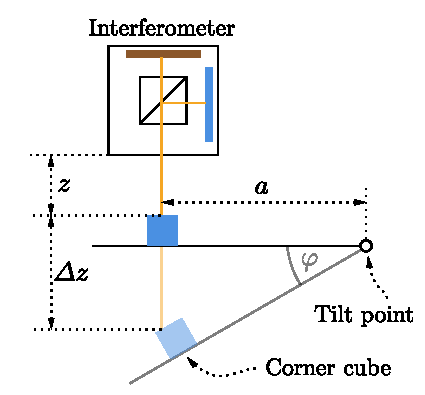
\includegraphics[width=0.8\textwidth]{figures/abbeerror.pdf}
	\caption{Visualization of a so-called Abbe offset error $\Delta z$.}
	\label{fig:abbeerror}
      \end{figure}
    \end{column}
  \end{columns}
\end{frame}

\begin{frame}[allowframebreaks]{Hypotheses}
  \framesubtitle{Hypothesis and aim 2}

  \begin{columns}
    \begin{column}{0.49\textwidth}
    Text.
    \end{column}
    
    \begin{column}{0.5\textwidth}
      \begin{figure}[h!] 
	\centering
	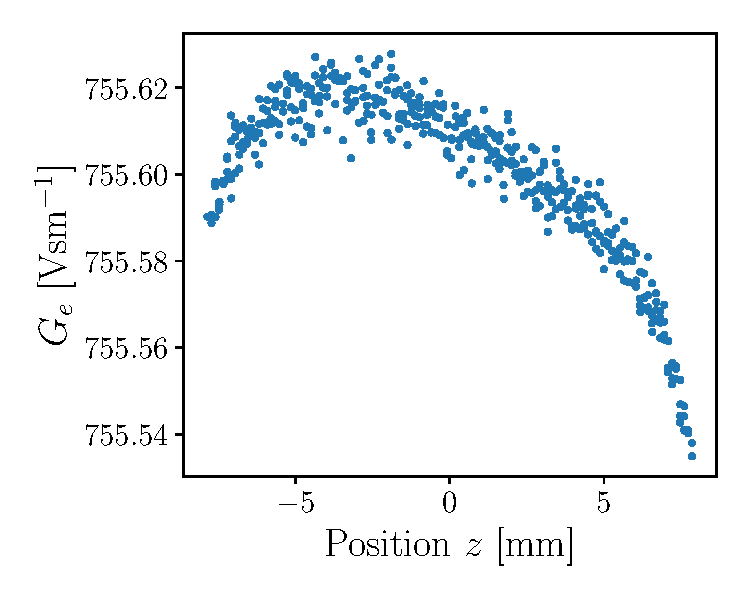
\includegraphics[width=0.8\textwidth]{figures/Ge_example.pdf}
	\caption{Example datapoints obtained for the $G_e = U_d/v$ profile.}
	\label{fig:U_d_over_v_profile}
      \end{figure}
    \end{column}
  \end{columns}
\end{frame}

\begin{frame}[allowframebreaks]{Hypotheses}
  \framesubtitle{Hypothesis and aim 3}

  \begin{columns}
    \begin{column}{0.49\textwidth}
    Text.
    \end{column}
    
    \begin{column}{0.5\textwidth}
    Text.
    \end{column}
  \end{columns}
\end{frame}

\begin{frame}[allowframebreaks]{Hypotheses}
  \framesubtitle{Hypothesis and aim 4}

  \begin{columns}
    \begin{column}{0.49\textwidth}
    Text.
    \end{column}
    
    \begin{column}{0.5\textwidth}
      \begin{figure}[h!] 
	\centering
	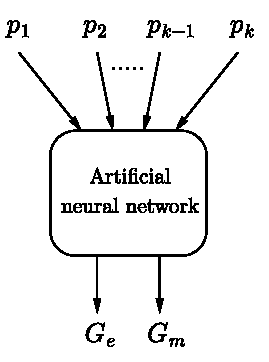
\includegraphics[width=0.6\textwidth]{figures/nn.pdf}
	\caption{Proposed architecture of the neural network; $\vect{p}$ are the alignment parameters and $\vect{q}$ are the geometrical factors associated to the alignment parameters.}
	\label{fig:nn}
      \end{figure}
    \end{column}
  \end{columns}
\end{frame}

\section{Methods and research plan}
\begin{frame}[allowframebreaks]{Methods and research plan}
  \framesubtitle{Milestones}
    Text.
\end{frame}

\begin{frame}[allowframebreaks]{Methods and research plan}
  \framesubtitle{Anticipated problems and possible solutions}
  Text.
\end{frame}

\section{Significance}
\begin{frame}[allowframebreaks]{Significance}
  \framesubtitle{Significance of the proposed project}
    Text.
\end{frame}

\section*{Literature}
\begin{frame}[allowframebreaks]{Literature}
\scriptsize
\bibliography{references}
\bibliographystyle{apalike}
\nocite{Eichenberger_2022}
\nocite{Fang_2020}
\nocite{Haddad_2017}
\nocite{Kibble1976}
\nocite{Stock_2023}
\nocite{Xu_2016}
\end{frame}

\section*{Questions}
\begin{frame}[allowframebreaks]{Questions}
Thank you for your time and attention!
\end{frame}

\appendix

\section*{Appendix}
\begin{frame}[allowframebreaks]{Appendix}
\framesubtitle{Maxwell's equations}
\justifying
Consider an electric field $\vect{E}(\vect{r},t)$, a magnetic field $\vect{B}(\vect{r},t)$, a charge density $\rho(\vect{r},t)$ and a current density $\vect{j}(\vect{r},t)$. The four so-called Maxwell equations \begin{equation}\scriptsize
	\vect{\nabla}\cdot \vect{E} = \frac{\rho}{\epsilon_0} \quad \Leftrightarrow \quad \oint_{\partial V} \vect{E}\cdot \mathrm{d}\vect{S} = \frac{1}{\epsilon_0}\int_{V}\rho\,\mathrm{d}V
	\end{equation}
	\begin{equation}\scriptsize
	\vect{\nabla}\cdot \vect{B} = 0 \quad \Leftrightarrow \quad \oint_{\partial V}\vect{B}\cdot \mathrm{d}\vect{S} = 0
	\end{equation}
	\begin{equation}\scriptsize
	\vect{\nabla} \times \vect{E} = - \frac{\partial \vect{B}}{\partial t} \quad \Leftrightarrow \quad \oint_{\partial S}\vect{E}\cdot \mathrm{d}\vect{l} = -\int_{S}\frac{\partial \vect{B}}{\partial t}\cdot \mathrm{d}\vect{S}
	\end{equation}
	\begin{equation}\scriptsize
	\vect{\nabla} \times \vect{B} = \mu_0\vect{j} + \mu_0\epsilon_0\frac{\partial \vect{E}}{\partial t} \quad \Leftrightarrow \quad \oint_{\partial S}\vect{B}\cdot \mathrm{d}\vect{l} = \mu_0\int_{S}\vect{j}\cdot \mathrm{d}\vect{S} + \mu_0\epsilon_0\int_{S}\frac{\partial \vect{E}}{\partial t}\cdot \mathrm{d}\vect{S}
	\end{equation} govern these physical quantities.
\end{frame}

\begin{frame}[allowframebreaks]{Appendix}
\framesubtitle{Electromagnetic induction}
\justifying
 In order to derive an expression for electromagnetic induction, it is necessary to invoke Maxwell's equations; in particular the Lorentz force equation \begin{equation}
		\vect{F}(\vect{r}, t) = q\left[\vect{E}(\vect{r},t) + \vect{v}(t)\times \vect{B}(\vect{r},t)\right],
	\end{equation} where $\vect{r}$ and $t$ denote the position and time of evaluation; and where $q$ is a charge probe, $\vect{v}$ is the velocity of $q$ and $\vect{E}$ and $\vect{B}$ are the electric and magnetic field respectively. Furthermore, the third Maxwell equation is of interest for the watt and joule balance techniques, namely \begin{equation}\label{eq:maxwell3rd_diff}
	\vect{\nabla} \times \vect{E}(\vect{r},t) = -\frac{\partial \vect{B}(\vect{r},t)}{\partial t}.
	\end{equation}
	
	\pagebreak In addition to these equations, also the integral theorem of Stokes is relevant; let $\Sigma$ denote an arbitrary surfae in $\mathbb{R}^3$ and let $\partial \Sigma$ denote its boundary, which in this case is a line in $\mathbb{R}^3$. If then $\vect{V}$ is an arbitrary vector field in $\mathbb{R}^3$, the integral theorem of Stokes states that \begin{equation}
		\int_{\Sigma} (\vect{\nabla} \times \vect{V})\cdot \mathrm{d}\vect{S} = \oint_{\partial \Sigma} \vect{V}\cdot \mathrm{d}\vect{l},
	\end{equation} where $\mathrm{d}\vect{S}$ denotes the oriented surface element of $\Sigma$ and $\mathrm{d}\vect{l}$ is a line element of $\partial \Sigma$. With this theorem, Maxwell's third equation \cref{eq:maxwell3rd_diff} can be transformed to the integral form \begin{equation}
	\label{eq:maxwell3rd_int}
	\oint_{\partial \Sigma} \vect{E}(\vect{r},t)\cdot \mathrm{d}\vect{l} = -\int_{\Sigma} \frac{\partial \vect{B}(\vect{r},t)}{\partial t}\cdot \mathrm{d}\vect{S}.
	\end{equation}
	
  \pagebreak
 If the surface $\Sigma$ becomes time-dependent $\Sigma \rightarrow \Sigma(t)$, the magnetic flux $\Phi_B$ through the surface $\Sigma(t)$ can be written as \begin{equation}
		\Phi_B = \int_{\Sigma(t)} \vect{B}(\vect{r},t)\cdot \mathrm{d}\vect{S}.
	\end{equation} The total time derivative of the magnetic flux in turn gives the negative induced voltage $U(t)$, namely \begin{equation}
	U(t) = -\frac{\mathrm{d}\Phi_B}{\mathrm{d}t} = -\frac{\mathrm{d}}{\mathrm{d}t} \int_{\Sigma(t)} \vect{B}(\vect{r},t)\cdot \mathrm{d}\vect{S}.
	\end{equation} In order to evaluate this total time derivative, both a change in the magnetic field aswell as in the surface element have to be considered. The change in the surface element $\mathrm{d}\vect{S}$ with time $t$ can be written as $\tfrac{\mathrm{d}\vect{S}}{\mathrm{d}t} = \vect{v} \times \mathrm{d}\vect{l}$, as \cref{fig:changeinsurfaceelement} indicates.
	\begin{figure}[h]
		\centering
		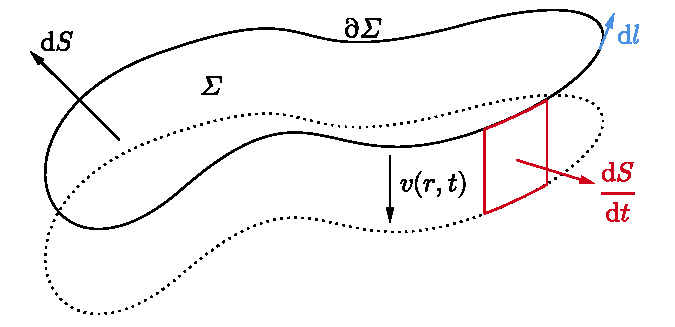
\includegraphics[width=0.6\textwidth]{figures/changeinsurfaceelement}
		\caption{Illustration for the derivation of the expression for the change in the surface element $\tfrac{\mathrm{d}\vect{S}}{\mathrm{d}t} = \vect{v} \times \mathrm{d}\vect{l}$.}
		\label{fig:changeinsurfaceelement}
	\end{figure}
	With this knowledge, one can differentiate both $\vect{B}(\vect{r},t)$ and $\mathrm{d}\vect{S}$ in the integrand to arrive at \begin{align}
		\begin{aligned}
			\frac{\mathrm{d}\Phi_B}{\mathrm{d}t} &= \frac{\mathrm{d}}{\mathrm{d}t} \int_{\Sigma(t)}\vect{B}(\vect{r},t)\cdot \mathrm{d}\vect{S} \\
			&= \int_{\Sigma(t)}\frac{\partial \vect{B}(\vect{r},t)}{\partial t}\cdot \mathrm{d}\vect{S} + \int_{\Sigma(t)}\vect{B}(\vect{r},t)\cdot \frac{\mathrm{d}\vect{S}}{\mathrm{d}t} \\
			&= - \oint_{\partial \Sigma(t)} \vect{E}(\vect{r},t)\cdot \mathrm{d}\vect{l} + \oint_{\partial \Sigma(t)}\vect{B}(\vect{r},t)\cdot (\vect{v}(t)\times \mathrm{d}\vect{l}) \\
			&= -\oint_{\partial \Sigma(t)} \left[\vect{E}(\vect{r},t) + \vect{v}(t) \times \vect{B}(\vect{r},t)\right]\cdot \mathrm{d}\vect{l} = -U(t).
		\end{aligned}
	\end{align} In the case where the external magnetic field is zero, i.e. $\vect{E}(\vect{r},t) = 0$, this equation reduces to \begin{equation}\label{eq:watt_bal_fund_eq_1}
	U(t) = \oint_{\partial \Sigma(t)} \left[\vect{v}(t) \times \vect{B}(\vect{r},t)\right]\cdot \mathrm{d}\vect{l}
	\end{equation} and is herewith the first of the fundamental equations used for the Kibble balance experiment.
\end{frame}

\begin{frame}[allowframebreaks]{Appendix}
\framesubtitle{Electromagnetic force}
\justifying
	A second important equation is derived from the Lorentz force equation. Consider for this purpose \cref{fig:lorentzforceeq}. \begin{figure}[h]
	\centering
	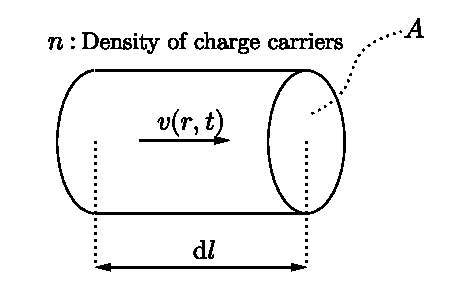
\includegraphics[width=0.4\textwidth]{figures/lorentzforceeq.pdf}
	\caption{Illustration to derive the second important equation needed for the Kibble balance principle.}
	\label{fig:lorentzforceeq}
	\end{figure}
	In this figure, a short element of length $\mathrm{d}l$ of a wire with charge carrier density $n$ is shown. In principle, this wire represents any object of choice. If one assumes, that this wire or alternatively an object of choice is immersed in a magnetic field $\vect{B}(\vect{r},t)$, a magnetic force is exerted on charge carriers moving at speed $\vect{v}(t)$ in the object. Assuming that all charge carriers move at speed $\vect{v}(t)$, the total current $I(t)$ is given by $I(t) = nAe|\vect{v}(t)$. 
 
 \pagebreak 
 
 The electromagnetic force exerted on one electron would be given by the expression $e\vect{E}(\vect{r},t) + e\vect{v}(t) \times \vect{B}(\vect{r},t)$; and on $nA\,\mathrm{d}l$ carriers with no external electric field ($\vect{E}(\vect{r},t) = 0$), the force differential $\mathrm{d}\vect{F}$ is given by 
 \begin{align}\begin{aligned}
		\mathrm{d}\vect{F} = neA\,\mathrm{d}l \left[\vect{v}(t)\times \vect{B}(\vect{r},t)\right] &= I(t)\,\mathrm{d}\vect{l}\times \vect{B}(\vect{r},t) \\ &= -I(t)\vect{B}(\vect{r},t)\times \mathrm{d}\vect{l},
	\end{aligned}\end{align} where in the last steps the definition $\mathrm{d}\vect{l} \doteq \mathrm{d}l\frac{\vect{v}}{|\vect{v}|}$ was used. Integrated over a closed path $\partial \Sigma(t)$ therefore one obtains the magnetic force on the object given by \begin{equation}\label{eq:watt_bal_fund_eq_2}
	\vect{F}(\vect{r},t) = -I(t)\oint_{\partial \Sigma(t)} \vect{B}(\vect{r},t)\times \mathrm{d}\vect{l}.
	\end{equation}
\end{frame}

\begin{frame}[allowframebreaks]{Appendix}
\framesubtitle{Quantum Hall effect}
\justifying
	The quantum Hall effect can be used for resistance measurement; according to \cite{B_Jeckelmann_2001}, the quantum Hall resistance $R_H$ is given by the expression \begin{equation}\label{eq:quantumhalleffect}
		R_H = \frac{h}{n_He^2}, \quad n_H \in \mathbb{N},
	\end{equation} where $h = \SI{6.62607015e-35}{\joule\second}$ is the Planck constant and $e$ is the elementary charge.
\end{frame}

\begin{frame}[allowframebreaks]{Appendix}
\framesubtitle{Josephson effect}
\justifying
	The Josephson voltage $U_J$ across a Josephson junction can be used for voltage measurements; according to \cite{Kajastie_2009} it is given by the equation \begin{equation}\label{eq:josephsoneffect}
		U_J = \frac{2e}{h}n_Jf_J, \quad n_J \in \mathbb{N},
	\end{equation} where $h$ is the Planck constant, $e$ is the elementary charge and $f_J$ is the frequency of the microwave radiation used to irradiate the Josephson junction with.
\end{frame}

\end{document}
